% Compile with: latexmk -pdf 1.1_fem_foundations.tex
% Figures are read from ./figures; missing images use TikZ fallbacks.
\documentclass[aspectratio=169,11pt]{beamer}
\usetheme{default}
\usepackage[T1]{fontenc}
\usepackage{lmodern}
\usepackage{amsmath,amssymb,mathtools,bm}
\usepackage{booktabs,graphicx,xcolor,adjustbox}
\usepackage{tikz,pgfplots}
\usetikzlibrary{positioning,calc,arrows.meta}
\pgfplotsset{compat=1.18}
\definecolor{FEMnavy}{HTML}{17365D}
\definecolor{FEMblue}{HTML}{2B6CB0}
\definecolor{FEMteal}{HTML}{1597A5}
\definecolor{FEMorange}{HTML}{D7653B}
\definecolor{FEMlight}{HTML}{F4F7FA}
\definecolor{FEMgray}{HTML}{5C6F82}
\definecolor{FEMpale}{HTML}{EAF7F9}
\definecolor{FEMcream}{HTML}{FFF4EA}
\setbeamercolor{normal text}{fg=FEMnavy,bg=white}
\setbeamercolor{structure}{fg=FEMblue}
\setbeamercolor{frametitle}{fg=white,bg=FEMnavy}
\setbeamercolor{title}{fg=white}
\setbeamercolor{block title}{fg=white,bg=FEMblue}
\setbeamercolor{block body}{fg=FEMnavy,bg=FEMlight}
\setbeamercolor{alerted text}{fg=FEMorange}
\setbeamercolor{block title alerted}{fg=white,bg=FEMorange}
\setbeamercolor{block body alerted}{fg=FEMnavy,bg=FEMcream}
\setbeamercolor{block title example}{fg=white,bg=FEMteal}
\setbeamercolor{block body example}{fg=FEMnavy,bg=FEMpale}
\setbeamercolor{key line}{fg=FEMnavy,bg=FEMpale}
\setbeamertemplate{navigation symbols}{}
\setbeamertemplate{itemize item}{\color{FEMteal}$\blacktriangleright$}
\setbeamertemplate{itemize subitem}{\color{FEMteal}$\bullet$}
\setbeamertemplate{frametitle}{\nointerlineskip\begin{beamercolorbox}[wd=\paperwidth,ht=.82cm,dp=.25cm,leftskip=.55cm]{frametitle}\usebeamerfont{frametitle}\insertframetitle\end{beamercolorbox}}
\setbeamertemplate{footline}{\leavevmode\hbox{\begin{beamercolorbox}[wd=.82\paperwidth,ht=2.6ex,dp=1.1ex,leftskip=.55cm]{author in head/foot}\color{FEMgray}\scriptsize Finite Element Methods: Foundations\end{beamercolorbox}\begin{beamercolorbox}[wd=.18\paperwidth,ht=2.6ex,dp=1.1ex,rightskip=.55cm plus1fil]{date in head/foot}\color{FEMgray}\scriptsize\hfill\insertframenumber/\inserttotalframenumber\end{beamercolorbox}}}
\setbeamersize{text margin left=.65cm,text margin right=.65cm}
\setbeamerfont{frametitle}{size=\Large,series=\bfseries}
\setbeamerfont{itemize/enumerate body}{size=\normalsize}
\setbeamerfont{itemize/enumerate subbody}{size=\normalsize}
\setbeamerfont{block body}{size=\normalsize}
\setbeamerfont{block title}{size=\normalsize,series=\bfseries}
\setlength{\leftmargini}{1.25em}
\addtobeamertemplate{itemize/enumerate body begin}{\setlength\itemsep{.75em}}{}
\setlength{\parskip}{.45em}
\newcommand{\key}[1]{\par\vspace{4mm}\begin{beamercolorbox}[sep=2.5mm,wd=\textwidth]{key line}\normalsize #1\end{beamercolorbox}}
\newcommand{\FEMfigure}[3][.65\textheight]{%
\begin{center}\IfFileExists{#2}{\includegraphics[width=\linewidth,height=#1,keepaspectratio]{#2}}{\begin{adjustbox}{max width=\linewidth,max totalheight=#1}#3\end{adjustbox}}\end{center}}
% Use one supplied panel on introductory slides; retain the full comparison later.
\newcommand{\FEMfigurecropped}[4][.65\textheight]{%
\begin{center}\IfFileExists{#2}{\includegraphics[trim=#3,clip,width=\linewidth,height=#1,keepaspectratio]{#2}}{\begin{adjustbox}{max width=\linewidth,max totalheight=#1}#4\end{adjustbox}}\end{center}}
% Figures live in ./figures. \IfFileExists (used above) searches \input@path,
% \includegraphics searches \graphicspath.
\graphicspath{{figures/}}
\makeatletter\def\input@path{{figures/}}\makeatother
\newcommand{\R}{\mathbb R}
\newcommand{\Oh}{\Omega}
\title{Finite Element Methods: Foundations}
\subtitle{From weak forms to error estimates}
\author{}
\date{}
\hypersetup{pdftitle={Finite Element Methods: Foundations},pdfsubject={Lecture slides},pdfauthor={}}
\begin{document}
\section{Motivation and roadmap}
\begin{frame}[plain]
\begin{tikzpicture}[remember picture,overlay]
\IfFileExists{a_wide_cinematic_high_detail_digital_illustratio.png}{
\node[inner sep=0pt] at (current page.center) {\includegraphics[width=\paperwidth,height=\paperheight]{a_wide_cinematic_high_detail_digital_illustratio.png}};
\fill[FEMnavy,opacity=.82] (current page.south west) rectangle (current page.north east);
}{
\fill[FEMnavy] (current page.south west) rectangle (current page.north east);
\begin{scope}[shift={(current page.south east)},x=1cm,y=1cm]
\foreach \x in {-6,-4.7,-3.4,-2.1,-.8}{\foreach \y in {.1,1.4,2.7,4,5.3,6.6}{
\draw[white,opacity=.10] (\x,\y) rectangle ++(1.3,1.3);
\draw[white,opacity=.10] (\x,\y)--++(1.3,1.3);}}
\end{scope}}
\node[anchor=west,text width=12.7cm] at ([xshift=.85cm,yshift=.55cm]current page.west) {
{\color{FEMteal!70!white}\large\bfseries FROM PHYSICAL LAWS TO SIMULATIONS}\\[7mm]
{\color{white}\fontsize{29}{34}\selectfont\bfseries Finite Element Methods:\\Foundations}\\[5mm]
{\color{white!80}\Large From weak forms to error estimates}};
\node[anchor=south west,text=white!70] at ([xshift=.85cm,yshift=.72cm]current page.south west)
{Weak forms\quad$\longrightarrow$\quad finite elements\quad$\longrightarrow$\quad reliable solutions};
\end{tikzpicture}
\end{frame}

\begin{frame}{Why FEM?}
\begin{columns}[c,onlytextwidth]\column{.43\textwidth}
\begin{block}{Real models are rarely simple}
\begin{itemize}
\item Complicated geometry and material variation.
\item Fields such as temperature, displacement, and pressure.
\end{itemize}
\end{block}
\column{.53\textwidth}
\begin{exampleblock}{FEM makes them computable}
\begin{itemize}
\item Local polynomial approximations on a mesh.
\item Sparse systems with a route to error control.
\end{itemize}
\end{exampleblock}
\end{columns}
\key{Along with the solution, we need an estimate of its error.}
\end{frame}

\begin{frame}{From a PDE to a simulation}
\begin{center}
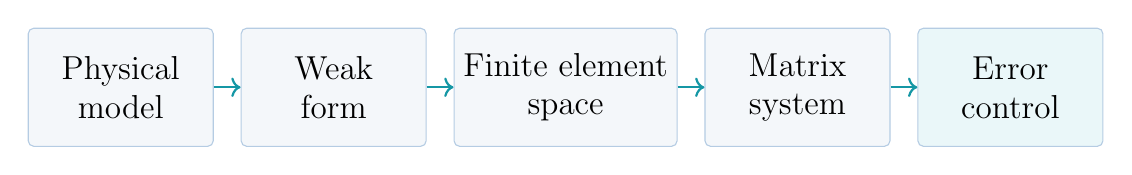
\begin{tikzpicture}[node distance=.34cm]
\tikzset{stage/.style={draw=FEMblue!35,fill=FEMlight,rounded corners=2pt,minimum width=2.35cm,minimum height=1.5cm,align=center,font=\large}}
\node[stage] (a) {Physical\\model};
\node[stage,right=of a] (b) {Weak\\form};
\node[stage,right=of b] (c) {Finite element\\space};
\node[stage,right=of c] (d) {Matrix\\system};
\node[stage,fill=FEMpale,right=of d] (e) {Error\\control};
\foreach \a/\b in {a/b,b/c,c/d,d/e}{\draw[->,FEMteal,thick] (\a)--(\b);}
\end{tikzpicture}
\end{center}
\vspace{5mm}
\begin{center}\large One model problem will connect every step.\end{center}
\end{frame}

\begin{frame}{Our model problem}
\begin{block}{Poisson equation}
\[
-\Delta u=f\quad\text{in }\Omega,\qquad u=0\quad\text{on }\partial\Omega.
\]
\end{block}\begin{columns}[c,onlytextwidth]\column{.43\textwidth}
\begin{itemize}
\item $u$: the unknown field.
\item $f$: the prescribed source.
\end{itemize}
\column{.53\textwidth}
\begin{exampleblock}{Why this example?}
We can derive its weak form, assemble its stiffness matrix, and estimate the error.
\end{exampleblock}
\end{columns}
\end{frame}

\section{Weak formulations and well-posedness}
\begin{frame}{A warm-up in one dimension}
\begin{block}{Start with the differential equation}
\[
-u''=f\quad\text{on }(0,1),\qquad u(0)=u(1)=0.
\]
\end{block}\begin{itemize}
\item Multiply by a test function $v$ with $v(0)=v(1)=0$.
\item Integrate over the interval.
\end{itemize}\[
\int_0^1(-u'')v\,dx=\int_0^1fv\,dx.
\]
\end{frame}

\begin{frame}{Integration by parts}
\[
\int_0^1(-u'')v\,dx=\int_0^1u'v'\,dx-\big[u'v\big]_0^1.
\]\begin{exampleblock}{The test function vanishes at both ends}
\[
\boxed{\int_0^1u'v'\,dx=\int_0^1fv\,dx.}
\]
\end{exampleblock}\key{Integration by parts leaves only first derivatives of $u$ and $v$.}
\end{frame}

\begin{frame}{The weak Poisson problem}
Find $u\in V=H_0^1(\Omega)$ such that\[
\boxed{\int_\Omega\nabla u\cdot\nabla v\,dx=\int_\Omega f v\,dx\qquad\forall v\in V.}
\]\begin{columns}[c,onlytextwidth]\column{.43\textwidth}
\begin{block}{Energy form}
\[
a(u,v)=\int_\Omega\nabla u\cdot\nabla v\,dx.
\]
\end{block}
\column{.53\textwidth}
\begin{exampleblock}{Load functional}
\[
\ell(v)=\int_\Omega fv\,dx.
\]
\end{exampleblock}
\end{columns}\centering We write this as $a(u,v)=\ell(v)$.
\end{frame}

\begin{frame}{What belongs to the function space?}
\begin{block}{$H_0^1(\Omega)$}
\begin{itemize}
\item The function and its first weak derivatives are square integrable.
\item Its boundary value is zero in the trace sense.
\end{itemize}
\end{block}\begin{exampleblock}{Why this matters for FEM}
Continuous piecewise-linear functions can belong to this space even though their gradients jump between cells.
\end{exampleblock}
\end{frame}

\begin{frame}{Continuity and coercivity}
\begin{columns}[c,onlytextwidth]\column{.48\textwidth}
\begin{block}{Continuity: bounded response}
\[
|a(w,v)|\le M\|w\|_V\|v\|_V.
\]The constant $M$ bounds the size of $a(w,v)$.
\end{block}
\column{.48\textwidth}
\begin{exampleblock}{Coercivity: energy controls the norm}
\[
a(v,v)\ge\alpha\|v\|_V^2,\quad\alpha>0.
\]The energy controls the size of the function.
\end{exampleblock}
\end{columns}\key{Coercivity plays the role of positive definiteness.}
\end{frame}

\begin{frame}{Lax--Milgram: the result we use}
\begin{itemize}
\item $V$ is a Hilbert space.
\item $a$ is continuous and coercive.
\item $\ell$ is a continuous linear functional.
\end{itemize}\begin{exampleblock}{Existence, uniqueness, and stability}
There is a unique $u\in V$ with $a(u,v)=\ell(v)$ for every $v\in V$, and\[
\boxed{\|u\|_V\le\alpha^{-1}\|\ell\|_{V\prime}.}
\]
\end{exampleblock}
\end{frame}

\begin{frame}{Poisson satisfies the assumptions}
Use the energy norm $\|v\|_V=\|\nabla v\|_{L^2}$ on $H_0^1(\Omega)$.\[
\begin{aligned}|a(w,v)|&\le\|w\|_V\|v\|_V, && M=1,\\[2mm]a(v,v)&=\|v\|_V^2, &&\alpha=1.\end{aligned}
\]\begin{exampleblock}{The load is bounded}
For $f\in L^2(\Omega)$, Poincar\'e's inequality gives\[
|\ell(v)|\le C_P\|f\|_{L^2}\|v\|_V.
\]
\end{exampleblock}
\end{frame}

\begin{frame}{Mixed boundary data: where does the flux go?}
\begin{block}{A one-dimensional example}
\[
-u''=f,\qquad u(0)=0,\qquad u'(1)=g.
\]
\end{block}Choose test functions with $v(0)=0$, but do not require $v(1)=0$.\[
\boxed{\int_0^1u'v'\,dx=\int_0^1fv\,dx+g\,v(1).}
\]\key{Neumann data enter the load through the boundary term.}
\end{frame}

\begin{frame}{A simple well-posedness check}
For reaction--diffusion on $V=H^1(0,1)$, take\[
a(u,v)=\int_0^1u'v'\,dx+\int_0^1uv\,dx.
\]\begin{exampleblock}{Immediate energy identity}
\[
a(u,u)=\|u\|_{H^1}^2\qquad\Longrightarrow\qquad M=\alpha=1.
\]
\end{exampleblock}\begin{alertblock}{What changes without the mass term?}
On all of $H^1$, constant functions have zero gradient. Boundary conditions or another constraint are then needed for coercivity.
\end{alertblock}
\end{frame}

\section{Galerkin approximation}
\begin{frame}{From infinite to finite dimension}
\begin{columns}[c,onlytextwidth]\column{.48\textwidth}
\begin{block}{Continuous problem}
Find $u\in V$ with\[
a(u,v)=\ell(v)\quad\forall v\in V.
\]
\end{block}
\column{.48\textwidth}
\begin{exampleblock}{Galerkin problem}
Choose $V_h\subset V$ and find $u_h\in V_h$ with\[
a(u_h,v_h)=\ell(v_h)\quad\forall v_h\in V_h.
\]
\end{exampleblock}
\end{columns}\key{Keep the weak form. Restrict the trial and test space.}
\end{frame}

\begin{frame}{Stability passes to the discrete problem}
\begin{block}{Because $V_h\subset V$}
\begin{itemize}
\item The same continuity and coercivity bounds still hold.
\item The discrete problem therefore has a unique solution.
\end{itemize}
\end{block}\[
\|u_h\|_V\le\alpha^{-1}\|\ell\|_{V\prime}.
\]\key{The discrete problem is stable. Its accuracy depends on the choice of $V_h$.}
\end{frame}

\begin{frame}{Galerkin orthogonality}
Test both equations with the same $v_h\in V_h$ and subtract:\[
a(u,v_h)-a(u_h,v_h)=0.
\]\begin{exampleblock}{The key identity}
\[
\boxed{a(u-u_h,v_h)=0\qquad\forall v_h\in V_h.}
\]
\end{exampleblock}For the symmetric Poisson form, the error is orthogonal to $V_h$ in the energy inner product.
\end{frame}

\begin{frame}{C\'ea's lemma: nearly the best approximation}
For a continuous, coercive form and a conforming space $V_h\subset V$,\[
\boxed{\|u-u_h\|_V\le\frac{M}{\alpha}\inf_{v_h\in V_h}\|u-v_h\|_V.}
\]\begin{exampleblock}{Interpretation}
The FEM error is at most $M/\alpha$ times the best error in $V_h$.
\end{exampleblock}\key{To improve accuracy, improve the approximation space.}
\end{frame}

\begin{frame}{For Poisson: best approximation in energy}
The symmetric form defines $\|v\|_a^2=a(v,v)$.\[
\boxed{\|u-u_h\|_a=\min_{v_h\in V_h}\|u-v_h\|_a.}
\]\begin{exampleblock}{An energy projection}
Among all functions in $V_h$, the Galerkin solution is closest to $u$ in the energy norm.
\end{exampleblock}
\end{frame}

\section{Meshes and finite element spaces}
\begin{frame}{A first mesh in one dimension}
\begin{columns}[c,onlytextwidth]\column{.43\textwidth}
Split $[0,1]$ into elements $K_i=[x_{i-1},x_i]$.\[
h=\max_i|K_i|.
\]\begin{block}{For $P_1$}
The approximation is linear on each interval and determined by nodal values.
\end{block}
\column{.53\textwidth}
\FEMfigure[.67\textheight]{benchmark_a_coarse.png}{
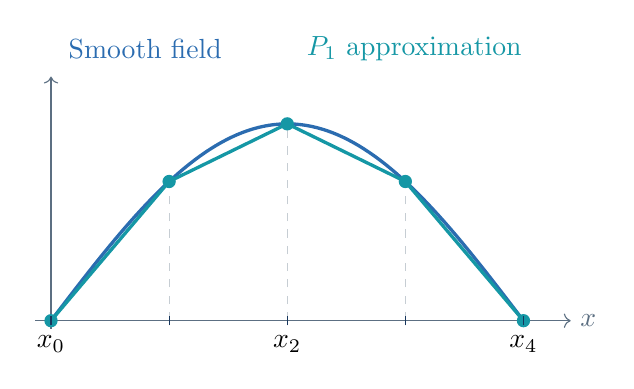
\begin{tikzpicture}[x=1cm,y=1cm]

\draw[->,FEMgray] (-.2,0)--(6.6,0) node[right] {$x$};
\draw[->,FEMgray] (0,-.1)--(0,3.1);
\draw[FEMblue,very thick,domain=0:6,samples=90] plot (\x,{2.5*sin(30*\x)});
\draw[FEMteal,very thick] (0,0)--(1.5,1.7678)--(3,2.5)--(4.5,1.7678)--(6,0);
\foreach \x/\y in {0/0,1.5/1.7678,3/2.5,4.5/1.7678,6/0}{
  \draw[FEMgray!35,dashed] (\x,0)--(\x,\y);
  \fill[FEMteal] (\x,\y) circle (2.4pt);
  \draw[FEMnavy] (\x,-.06)--(\x,.06);}
\node[below] at (0,-.07) {$x_0$}; \node[below] at (3,-.07) {$x_2$};
\node[below] at (6,-.07) {$x_4$};
\node[FEMblue,anchor=west] at (.1,3.45) {Smooth field};
\node[FEMteal,anchor=east] at (6.1,3.45) {$P_1$ approximation};

\end{tikzpicture}
}
\end{columns}
\end{frame}

\begin{frame}{A triangular mesh}
\begin{columns}[c,onlytextwidth]\column{.43\textwidth}
\begin{itemize}
\item The cells form a mesh $\mathcal T_h$.
\item Neighboring cells share a full edge or a vertex.
\item $h$ measures the largest cell size.
\end{itemize}
\column{.53\textwidth}
\FEMfigurecropped[.67\textheight]{mesh2d_gallery_slide.png}{0bp 0bp 489.6bp 0bp}{
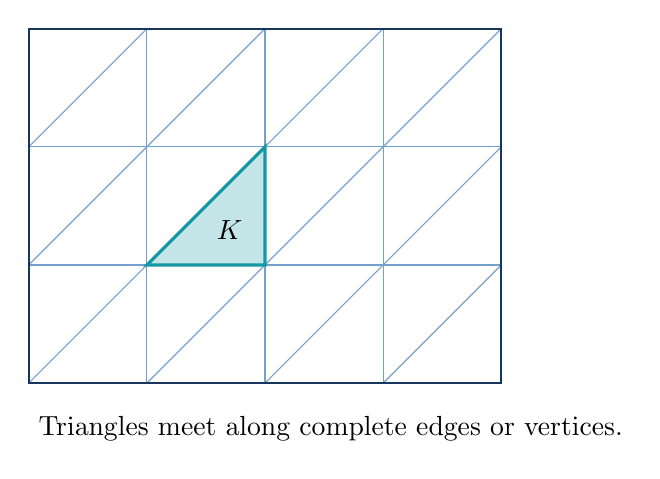
\begin{tikzpicture}[x=1cm,y=1cm]

\foreach \x in {0,1.5,3,4.5}{\foreach \y in {0,1.5,3}{
 \draw[FEMblue!65,thin] (\x,\y) rectangle ++(1.5,1.5);
 \draw[FEMblue!65,thin] (\x,\y)--++(1.5,1.5);}}
\fill[FEMteal!25] (1.5,1.5)--(3,1.5)--(3,3)--cycle;
\draw[FEMteal,very thick] (1.5,1.5)--(3,1.5)--(3,3)--cycle;
\draw[FEMnavy,thick] (0,0) rectangle (6,4.5);
\node at (2.55,1.95) {$K$};
\node[anchor=north west] at (0,-.3) {Triangles meet along complete edges or vertices.};

\end{tikzpicture}
}
\end{columns}
\end{frame}

\begin{frame}{Mesh quality is not just mesh size}
\FEMfigure[.56\textheight]{mesh2d_gallery_slide.png}{
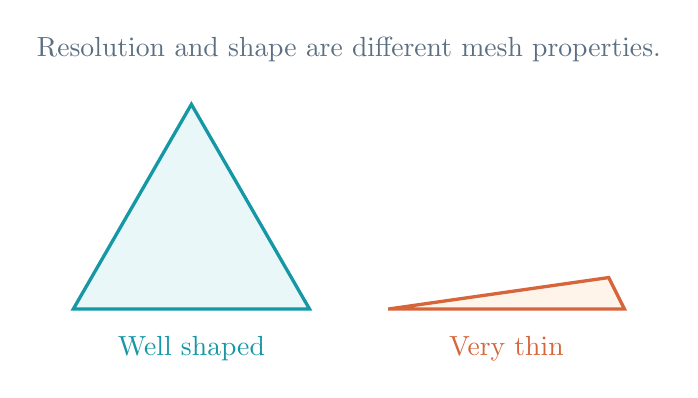
\begin{tikzpicture}[x=1cm,y=1cm]

\filldraw[fill=FEMpale,draw=FEMteal,very thick] (0,0)--(3,0)--(1.5,2.6)--cycle;
\filldraw[fill=FEMcream,draw=FEMorange,very thick] (4,0)--(7,0)--(6.8,.40)--cycle;
\node[FEMteal] at (1.5,-.5) {Well shaped};
\node[FEMorange] at (5.5,-.5) {Very thin};
\node[FEMgray,align=center] at (3.5,3.3) {Resolution and shape are different mesh properties.};

\end{tikzpicture}
}\key{Standard estimates assume shape-regular meshes: avoid arbitrarily thin cells.}
\end{frame}

\begin{frame}{What does $P_k$ mean?}
$P_k(K)$ contains polynomials of total degree at most $k$ on one cell.\begin{columns}[c,onlytextwidth]\column{.41\textwidth}
\begin{block}{$P_1$ on a triangle}
\[
p(x,y)=a+bx+cy.
\]Three coefficients.
\end{block}
\column{.55\textwidth}
\begin{exampleblock}{$P_2$ on a triangle}
\[
p(x,y)=a+bx+cy+dx^2+exy+fy^2.
\]Six coefficients.
\end{exampleblock}
\end{columns}\key{Raising the degree gives more freedom to approximate $u$ on the same cell.}
\end{frame}

\begin{frame}{Lagrange elements: the nodal idea}
\[
N_i(\xi_j)=\delta_{ij}.
\]\begin{columns}[c,onlytextwidth]\column{.47\textwidth}
\begin{block}{One node, one basis function}
A basis function is one at its own node and zero at the other nodes.
\end{block}
\column{.49\textwidth}
\begin{exampleblock}{Nodal values become coefficients}
\[
p(\xi)=\sum_i p(\xi_i)N_i(\xi).
\]
\end{exampleblock}
\end{columns}\key{The nodes determine the polynomial.}
\end{frame}

\begin{frame}{Two shape functions for a $P_1$ interval}
\begin{columns}[c,onlytextwidth]\column{.43\textwidth}
\[
\widehat\phi_0(\xi)=1-\xi,\qquad\widehat\phi_1(\xi)=\xi.
\]Two endpoint values determine one line.
\column{.53\textwidth}
\FEMfigure[.67\textheight]{lagrange_shape_functions_slide.png}{
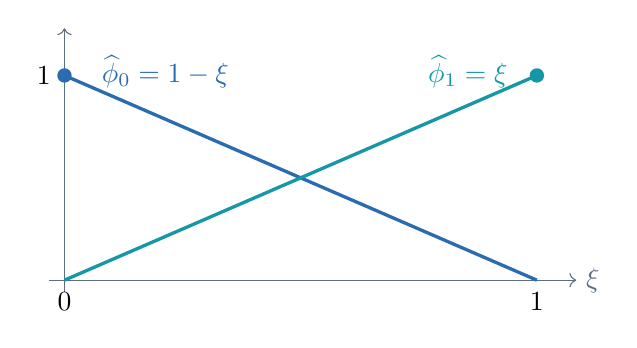
\begin{tikzpicture}[x=1cm,y=1cm]

\draw[->,FEMgray] (-.2,0)--(6.5,0) node[right] {$\xi$};
\draw[->,FEMgray] (0,-.15)--(0,3.2);
\draw[FEMblue,very thick] (0,2.6)--(6,0);
\draw[FEMteal,very thick] (0,0)--(6,2.6);
\foreach \x in {0,6}{\node[below] at (\x,-.04) {$\pgfmathparse{int(\x/6)}\pgfmathresult$};}
\fill[FEMblue] (0,2.6) circle (2.6pt); \fill[FEMteal] (6,2.6) circle (2.6pt);
\node[FEMblue,anchor=west] at (.35,2.65) {$\widehat\phi_0=1-\xi$};
\node[FEMteal,anchor=east] at (5.75,2.65) {$\widehat\phi_1=\xi$};
\node[anchor=east] at (-.05,2.6) {$1$};

\end{tikzpicture}
}
\end{columns}
\end{frame}

\begin{frame}{Global $P_1$: hat functions}
\begin{columns}[c,onlytextwidth]\column{.43\textwidth}
\[
\phi_i(x_j)=\delta_{ij}.
\]Each hat is supported on the two elements next to its node.\[
u_h=\sum_iU_i\phi_i,\qquad U_i=u_h(x_i).
\]
\column{.53\textwidth}
\FEMfigure[.67\textheight]{hat_functions.png}{
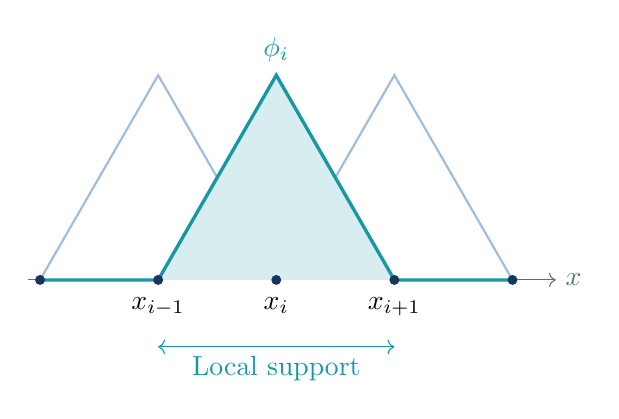
\begin{tikzpicture}[x=1cm,y=1cm]

\draw[->,FEMgray] (-.15,0)--(6.55,0) node[right] {$x$};
\foreach \x in {1.5,4.5}{\draw[FEMblue!45,thick] ({\x-1.5},0)--(\x,2.6)--({\x+1.5},0);}
\fill[FEMteal!17] (1.5,0)--(3,2.6)--(4.5,0)--cycle;
\draw[FEMteal,very thick] (0,0)--(1.5,0)--(3,2.6)--(4.5,0)--(6,0);
\foreach \x in {0,1.5,3,4.5,6}{\fill[FEMnavy] (\x,0) circle (1.8pt);}
\node[below] at (1.5,-.1) {$x_{i-1}$};\node[below] at (3,-.1) {$x_i$};\node[below] at (4.5,-.1) {$x_{i+1}$};
\node[FEMteal,above] at (3,2.65) {$\phi_i$};
\draw[<->,FEMteal] (1.5,-.85)--(4.5,-.85) node[midway,below] {Local support};

\end{tikzpicture}
}
\end{columns}
\end{frame}

\begin{frame}{$P_1$ on a triangle}
\begin{columns}[c,onlytextwidth]\column{.43\textwidth}
\begin{block}{Three vertex values}
A linear function $p(x,y)=a+bx+cy$ has three coefficients.
\end{block}Each local shape function is one at one vertex and zero at the other two.
\column{.53\textwidth}
\FEMfigurecropped[.67\textheight]{p1_p2_dof_layout_slide.png}{0bp 24.84bp 554.76bp 0bp}{
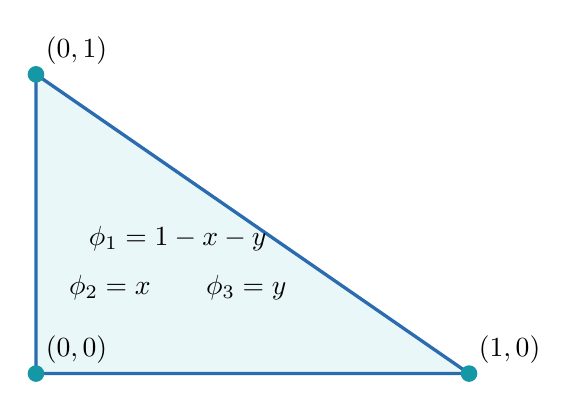
\begin{tikzpicture}[x=1cm,y=1cm]

\filldraw[fill=FEMpale,draw=FEMblue,very thick] (0,0)--(5.5,0)--(0,3.8)--cycle;
\foreach \x/\y/\label in {0/0/{(0,0)},5.5/0/{(1,0)},0/3.8/{(0,1)}}{
 \fill[FEMteal] (\x,\y) circle (3pt); \node[above right] at (\x,\y) {$\label$};}
\node[align=center] at (1.8,1.4) {$\phi_1=1-x-y$\\[2mm]$\phi_2=x\qquad \phi_3=y$};

\end{tikzpicture}
}
\end{columns}
\end{frame}

\begin{frame}{How local pieces form a conforming space}
\begin{itemize}
\item Use a polynomial on each cell.
\item Share nodal values across cell interfaces.
\item Set the boundary nodal values to zero.
\end{itemize}\[
\boxed{V_h\subset H_0^1(\Omega).}
\]\key{A conforming space lies inside the energy space, including its boundary conditions.}
\end{frame}

\begin{frame}{$P_1$ versus $P_2$: more information on each cell}
\FEMfigure[.62\textheight]{p1_p2_dof_layout_slide.png}{
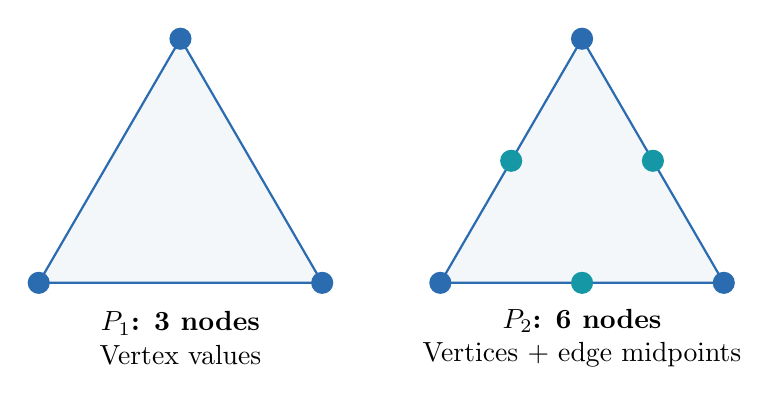
\begin{tikzpicture}[x=1cm,y=1cm]

\foreach \s in {0,5.1}{
 \filldraw[fill=FEMlight,draw=FEMblue,thick] (\s,0)--++(3.6,0)--++(-1.8,3.1)--cycle;
 \foreach \x/\y in {0/0,3.6/0,1.8/3.1}{\fill[FEMblue] ({\s+\x},\y) circle (4pt);}}
\foreach \x/\y in {6.9/0,6/1.55,7.8/1.55}{\fill[FEMteal] (\x,\y) circle (4pt);}
\node[align=center] at (1.8,-.7) {\textbf{$P_1$: 3 nodes}\\Vertex values};
\node[align=center] at (6.9,-.7) {\textbf{$P_2$: 6 nodes}\\Vertices + edge midpoints};

\end{tikzpicture}
}\key{Higher degree can improve accuracy for smooth solutions, but adds unknowns and cost.}
\end{frame}

\begin{frame}{Reference elements: reuse the same local construction}
\FEMfigure[.55\textheight]{isoparametric_geometry_slide.png}{
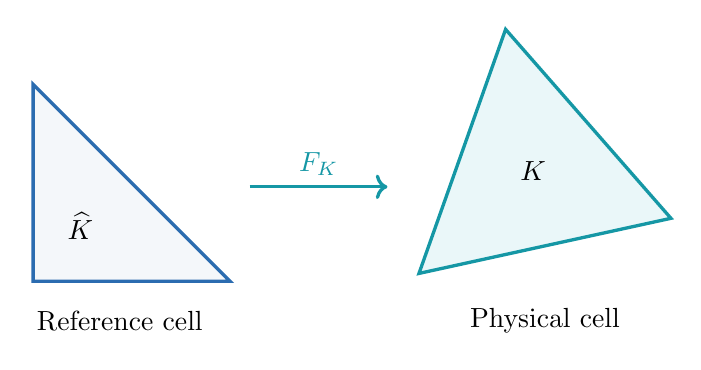
\begin{tikzpicture}[x=1cm,y=1cm]

\filldraw[fill=FEMlight,draw=FEMblue,very thick] (0,0)--(2.5,0)--(0,2.5)--cycle;
\node at (.6,.7) {$\widehat K$};
\draw[->,FEMteal,very thick] (2.75,1.2)--(4.5,1.2) node[midway,above] {$F_K$};
\filldraw[fill=FEMpale,draw=FEMteal,very thick] (4.9,.1)--(8.1,.8)--(6,3.2)--cycle;
\node at (6.35,1.4) {$K$};
\node at (1.1,-.5) {Reference cell};\node at (6.5,-.5) {Physical cell};

\end{tikzpicture}
}\begin{columns}[c,onlytextwidth]\column{.43\textwidth}
Define shape functions once on $\widehat K$.
\column{.53\textwidth}
Map them to each physical cell using $F_K$.
\end{columns}
\end{frame}

\section{Assembly and discrete systems}
\begin{frame}{From the weak form to a matrix system}
Expand the unknown and test with each basis function:\[
u_h=\sum_{j=1}^N U_j\phi_j\qquad\Longrightarrow\qquad\sum_{j=1}^N a(\phi_j,\phi_i)U_j=\ell(\phi_i).
\]\begin{exampleblock}{The linear system}
\[
\boxed{AU=F},\qquad A_{ij}=a(\phi_j,\phi_i),\quad F_i=\ell(\phi_i).
\]
\end{exampleblock}For Poisson, $A$ is the stiffness matrix.
\end{frame}

\begin{frame}{One element stiffness matrix}
On a $P_1$ interval of length $h_K$, the basis derivatives are $-1/h_K$ and $1/h_K$.\[
\boxed{A^K=\frac1{h_K}\begin{pmatrix}1&-1\\-1&1\end{pmatrix}.}
\]\key{Every entry is a local integral of two basis-function derivatives.}
\end{frame}

\begin{frame}{One element load vector}
For a constant source $f=1$ on an interval of length $h_K$,\[
F_m^K=\int_K\phi_m\,dx\qquad\Longrightarrow\qquad\boxed{F^K=\frac{h_K}{2}\begin{pmatrix}1\\1\end{pmatrix}.}
\]\begin{exampleblock}{Geometric interpretation}
Each basis function is a triangle of base $h_K$ and height one, so its integral is $h_K/2$.
\end{exampleblock}
\end{frame}

\begin{frame}{Local-to-global assembly}
\begin{columns}[c,onlytextwidth]\column{.43\textwidth}
\begin{itemize}
\item Compute a small matrix and load vector on each cell.
\item Map local node numbers to global unknowns.
\item Add contributions at shared unknowns.
\end{itemize}
\column{.53\textwidth}
\FEMfigure[.67\textheight]{hand_assembly_solution.png}{
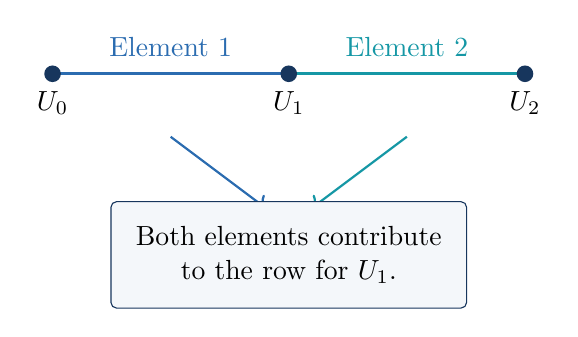
\begin{tikzpicture}[x=1cm,y=1cm]

\draw[FEMblue,very thick] (0,0)--(3,0);
\draw[FEMteal,very thick] (3,0)--(6,0);
\foreach \x/\n in {0/0,3/1,6/2}{\fill[FEMnavy] (\x,0) circle (3pt);\node[below] at (\x,-.1) {$U_{\n}$};}
\node[FEMblue,above] at (1.5,.1) {Element 1};\node[FEMteal,above] at (4.5,.1) {Element 2};
\draw[->,FEMblue,thick] (1.5,-.8)--(2.7,-1.7);
\draw[->,FEMteal,thick] (4.5,-.8)--(3.3,-1.7);
\node[draw=FEMnavy,fill=FEMlight,rounded corners=2pt,inner sep=9pt,align=center] at (3,-2.3)
 {Both elements contribute\\to the row for $U_1$.};

\end{tikzpicture}
}
\end{columns}
\end{frame}

\begin{frame}{Why the global matrix is sparse}
\FEMfigure[.55\textheight]{sparsity_pattern_slide.png}{
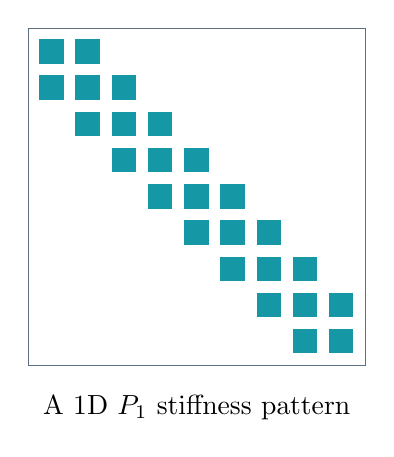
\begin{tikzpicture}[x=1cm,y=1cm]

\foreach \i in {0,...,8}{\foreach \j in {0,...,8}{
 \pgfmathtruncatemacro{\d}{abs(\i-\j)}
 \ifnum\d<2\fill[FEMteal] ({.46*\j},{-.46*\i}) rectangle ++(.31,-.31);\fi}}
\draw[FEMgray] (-.14,.14) rectangle (4.14,-4.14);
\node[below,align=center] at (2,-4.4) {A 1D $P_1$ stiffness pattern};

\end{tikzpicture}
}
\begin{block}{Only nearby basis functions interact}
\small
If $\phi_i$ and $\phi_j$ have no common cell of support, then $A_{ij}=0$.

Refinement enlarges the system without making every unknown interact with every other one.
\end{block}
\end{frame}

\begin{frame}{Boundary conditions in the discrete system}
\begin{columns}[c,onlytextwidth]\column{.48\textwidth}
\begin{block}{Dirichlet data}
\begin{itemize}
\item Fix the boundary nodal values.
\item For nonzero data, adjust the interior right-hand side.
\end{itemize}
\end{block}
\column{.48\textwidth}
\begin{exampleblock}{Neumann data}
\begin{itemize}
\item Keep the boundary flux term in the load.
\item Do not prescribe the corresponding field value.
\end{itemize}
\end{exampleblock}
\end{columns}\key{Impose the boundary conditions consistently with the weak form.}
\end{frame}

\begin{frame}{What a two-dimensional $P_1$ field looks like}
\FEMfigure[.64\textheight]{poisson2d_solution_slide.png}{
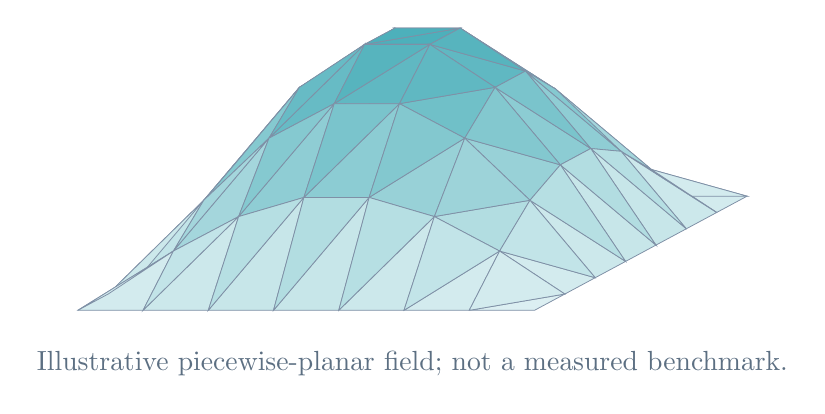
\begin{tikzpicture}[x=1cm,y=1cm]
\filldraw[fill=FEMteal!19!white,draw=FEMnavy!55,line width=.28pt] (2.3143,1.2429)--(3.1429,1.7888)--(3.5286,1.4500)--cycle;
\filldraw[fill=FEMteal!15!white,draw=FEMnavy!55,line width=.28pt] (2.3143,1.2429)--(3.5286,1.4500)--(2.7000,1.4500)--cycle;
\filldraw[fill=FEMteal!26!white,draw=FEMnavy!55,line width=.28pt] (3.1429,1.7888)--(3.9714,2.2266)--(4.3571,1.4500)--cycle;
\filldraw[fill=FEMteal!19!white,draw=FEMnavy!55,line width=.28pt] (3.1429,1.7888)--(4.3571,1.4500)--(3.5286,1.4500)--cycle;
\filldraw[fill=FEMteal!31!white,draw=FEMnavy!55,line width=.28pt] (3.9714,2.2266)--(4.8000,2.4696)--(5.1857,1.4500)--cycle;
\filldraw[fill=FEMteal!22!white,draw=FEMnavy!55,line width=.28pt] (3.9714,2.2266)--(5.1857,1.4500)--(4.3571,1.4500)--cycle;
\filldraw[fill=FEMteal!33!white,draw=FEMnavy!55,line width=.28pt] (4.8000,2.4696)--(5.6286,2.4696)--(6.0143,1.4500)--cycle;
\filldraw[fill=FEMteal!24!white,draw=FEMnavy!55,line width=.28pt] (4.8000,2.4696)--(6.0143,1.4500)--(5.1857,1.4500)--cycle;
\filldraw[fill=FEMteal!31!white,draw=FEMnavy!55,line width=.28pt] (5.6286,2.4696)--(6.4571,2.2266)--(6.8429,1.4500)--cycle;
\filldraw[fill=FEMteal!24!white,draw=FEMnavy!55,line width=.28pt] (5.6286,2.4696)--(6.8429,1.4500)--(6.0143,1.4500)--cycle;
\filldraw[fill=FEMteal!26!white,draw=FEMnavy!55,line width=.28pt] (6.4571,2.2266)--(7.2857,1.7888)--(7.6714,1.4500)--cycle;
\filldraw[fill=FEMteal!22!white,draw=FEMnavy!55,line width=.28pt] (6.4571,2.2266)--(7.6714,1.4500)--(6.8429,1.4500)--cycle;
\filldraw[fill=FEMteal!19!white,draw=FEMnavy!55,line width=.28pt] (7.2857,1.7888)--(8.1143,1.2429)--(8.5000,1.4500)--cycle;
\filldraw[fill=FEMteal!19!white,draw=FEMnavy!55,line width=.28pt] (7.2857,1.7888)--(8.5000,1.4500)--(7.6714,1.4500)--cycle;
\filldraw[fill=FEMteal!26!white,draw=FEMnavy!55,line width=.28pt] (1.9286,1.0357)--(2.7571,2.0195)--(3.1429,1.7888)--cycle;
\filldraw[fill=FEMteal!19!white,draw=FEMnavy!55,line width=.28pt] (1.9286,1.0357)--(3.1429,1.7888)--(2.3143,1.2429)--cycle;
\filldraw[fill=FEMteal!42!white,draw=FEMnavy!55,line width=.28pt] (2.7571,2.0195)--(3.5857,2.8084)--(3.9714,2.2266)--cycle;
\filldraw[fill=FEMteal!33!white,draw=FEMnavy!55,line width=.28pt] (2.7571,2.0195)--(3.9714,2.2266)--(3.1429,1.7888)--cycle;
\filldraw[fill=FEMteal!53!white,draw=FEMnavy!55,line width=.28pt] (3.5857,2.8084)--(4.4143,3.2462)--(4.8000,2.4696)--cycle;
\filldraw[fill=FEMteal!44!white,draw=FEMnavy!55,line width=.28pt] (3.5857,2.8084)--(4.8000,2.4696)--(3.9714,2.2266)--cycle;
\filldraw[fill=FEMteal!57!white,draw=FEMnavy!55,line width=.28pt] (4.4143,3.2462)--(5.2429,3.2462)--(5.6286,2.4696)--cycle;
\filldraw[fill=FEMteal!49!white,draw=FEMnavy!55,line width=.28pt] (4.4143,3.2462)--(5.6286,2.4696)--(4.8000,2.4696)--cycle;
\filldraw[fill=FEMteal!52!white,draw=FEMnavy!55,line width=.28pt] (5.2429,3.2462)--(6.0714,2.8084)--(6.4571,2.2266)--cycle;
\filldraw[fill=FEMteal!48!white,draw=FEMnavy!55,line width=.28pt] (5.2429,3.2462)--(6.4571,2.2266)--(5.6286,2.4696)--cycle;
\filldraw[fill=FEMteal!39!white,draw=FEMnavy!55,line width=.28pt] (6.0714,2.8084)--(6.9000,2.0195)--(7.2857,1.7888)--cycle;
\filldraw[fill=FEMteal!39!white,draw=FEMnavy!55,line width=.28pt] (6.0714,2.8084)--(7.2857,1.7888)--(6.4571,2.2266)--cycle;
\filldraw[fill=FEMteal!22!white,draw=FEMnavy!55,line width=.28pt] (6.9000,2.0195)--(7.7286,1.0357)--(8.1143,1.2429)--cycle;
\filldraw[fill=FEMteal!26!white,draw=FEMnavy!55,line width=.28pt] (6.9000,2.0195)--(8.1143,1.2429)--(7.2857,1.7888)--cycle;
\filldraw[fill=FEMteal!31!white,draw=FEMnavy!55,line width=.28pt] (1.5429,0.8286)--(2.3714,2.0553)--(2.7571,2.0195)--cycle;
\filldraw[fill=FEMteal!22!white,draw=FEMnavy!55,line width=.28pt] (1.5429,0.8286)--(2.7571,2.0195)--(1.9286,1.0357)--cycle;
\filldraw[fill=FEMteal!53!white,draw=FEMnavy!55,line width=.28pt] (2.3714,2.0553)--(3.2000,3.0390)--(3.5857,2.8084)--cycle;
\filldraw[fill=FEMteal!44!white,draw=FEMnavy!55,line width=.28pt] (2.3714,2.0553)--(3.5857,2.8084)--(2.7571,2.0195)--cycle;
\filldraw[fill=FEMteal!68!white,draw=FEMnavy!55,line width=.28pt] (3.2000,3.0390)--(4.0286,3.5850)--(4.4143,3.2462)--cycle;
\filldraw[fill=FEMteal!61!white,draw=FEMnavy!55,line width=.28pt] (3.2000,3.0390)--(4.4143,3.2462)--(3.5857,2.8084)--cycle;
\filldraw[fill=FEMteal!72!white,draw=FEMnavy!55,line width=.28pt] (4.0286,3.5850)--(4.8571,3.5850)--(5.2429,3.2462)--cycle;
\filldraw[fill=FEMteal!68!white,draw=FEMnavy!55,line width=.28pt] (4.0286,3.5850)--(5.2429,3.2462)--(4.4143,3.2462)--cycle;
\filldraw[fill=FEMteal!65!white,draw=FEMnavy!55,line width=.28pt] (4.8571,3.5850)--(5.6857,3.0390)--(6.0714,2.8084)--cycle;
\filldraw[fill=FEMteal!65!white,draw=FEMnavy!55,line width=.28pt] (4.8571,3.5850)--(6.0714,2.8084)--(5.2429,3.2462)--cycle;
\filldraw[fill=FEMteal!48!white,draw=FEMnavy!55,line width=.28pt] (5.6857,3.0390)--(6.5143,2.0553)--(6.9000,2.0195)--cycle;
\filldraw[fill=FEMteal!52!white,draw=FEMnavy!55,line width=.28pt] (5.6857,3.0390)--(6.9000,2.0195)--(6.0714,2.8084)--cycle;
\filldraw[fill=FEMteal!24!white,draw=FEMnavy!55,line width=.28pt] (6.5143,2.0553)--(7.3429,0.8286)--(7.7286,1.0357)--cycle;
\filldraw[fill=FEMteal!31!white,draw=FEMnavy!55,line width=.28pt] (6.5143,2.0553)--(7.7286,1.0357)--(6.9000,2.0195)--cycle;
\filldraw[fill=FEMteal!33!white,draw=FEMnavy!55,line width=.28pt] (1.1571,0.6214)--(1.9857,1.8481)--(2.3714,2.0553)--cycle;
\filldraw[fill=FEMteal!24!white,draw=FEMnavy!55,line width=.28pt] (1.1571,0.6214)--(2.3714,2.0553)--(1.5429,0.8286)--cycle;
\filldraw[fill=FEMteal!57!white,draw=FEMnavy!55,line width=.28pt] (1.9857,1.8481)--(2.8143,2.8319)--(3.2000,3.0390)--cycle;
\filldraw[fill=FEMteal!49!white,draw=FEMnavy!55,line width=.28pt] (1.9857,1.8481)--(3.2000,3.0390)--(2.3714,2.0553)--cycle;
\filldraw[fill=FEMteal!72!white,draw=FEMnavy!55,line width=.28pt] (2.8143,2.8319)--(3.6429,3.3778)--(4.0286,3.5850)--cycle;
\filldraw[fill=FEMteal!68!white,draw=FEMnavy!55,line width=.28pt] (2.8143,2.8319)--(4.0286,3.5850)--(3.2000,3.0390)--cycle;
\filldraw[fill=FEMteal!76!white,draw=FEMnavy!55,line width=.28pt] (3.6429,3.3778)--(4.4714,3.3778)--(4.8571,3.5850)--cycle;
\filldraw[fill=FEMteal!76!white,draw=FEMnavy!55,line width=.28pt] (3.6429,3.3778)--(4.8571,3.5850)--(4.0286,3.5850)--cycle;
\filldraw[fill=FEMteal!68!white,draw=FEMnavy!55,line width=.28pt] (4.4714,3.3778)--(5.3000,2.8319)--(5.6857,3.0390)--cycle;
\filldraw[fill=FEMteal!72!white,draw=FEMnavy!55,line width=.28pt] (4.4714,3.3778)--(5.6857,3.0390)--(4.8571,3.5850)--cycle;
\filldraw[fill=FEMteal!49!white,draw=FEMnavy!55,line width=.28pt] (5.3000,2.8319)--(6.1286,1.8481)--(6.5143,2.0553)--cycle;
\filldraw[fill=FEMteal!57!white,draw=FEMnavy!55,line width=.28pt] (5.3000,2.8319)--(6.5143,2.0553)--(5.6857,3.0390)--cycle;
\filldraw[fill=FEMteal!24!white,draw=FEMnavy!55,line width=.28pt] (6.1286,1.8481)--(6.9571,0.6214)--(7.3429,0.8286)--cycle;
\filldraw[fill=FEMteal!33!white,draw=FEMnavy!55,line width=.28pt] (6.1286,1.8481)--(7.3429,0.8286)--(6.5143,2.0553)--cycle;
\filldraw[fill=FEMteal!31!white,draw=FEMnavy!55,line width=.28pt] (0.7714,0.4143)--(1.6000,1.3980)--(1.9857,1.8481)--cycle;
\filldraw[fill=FEMteal!24!white,draw=FEMnavy!55,line width=.28pt] (0.7714,0.4143)--(1.9857,1.8481)--(1.1571,0.6214)--cycle;
\filldraw[fill=FEMteal!52!white,draw=FEMnavy!55,line width=.28pt] (1.6000,1.3980)--(2.4286,2.1869)--(2.8143,2.8319)--cycle;
\filldraw[fill=FEMteal!48!white,draw=FEMnavy!55,line width=.28pt] (1.6000,1.3980)--(2.8143,2.8319)--(1.9857,1.8481)--cycle;
\filldraw[fill=FEMteal!65!white,draw=FEMnavy!55,line width=.28pt] (2.4286,2.1869)--(3.2571,2.6248)--(3.6429,3.3778)--cycle;
\filldraw[fill=FEMteal!65!white,draw=FEMnavy!55,line width=.28pt] (2.4286,2.1869)--(3.6429,3.3778)--(2.8143,2.8319)--cycle;
\filldraw[fill=FEMteal!68!white,draw=FEMnavy!55,line width=.28pt] (3.2571,2.6248)--(4.0857,2.6248)--(4.4714,3.3778)--cycle;
\filldraw[fill=FEMteal!72!white,draw=FEMnavy!55,line width=.28pt] (3.2571,2.6248)--(4.4714,3.3778)--(3.6429,3.3778)--cycle;
\filldraw[fill=FEMteal!61!white,draw=FEMnavy!55,line width=.28pt] (4.0857,2.6248)--(4.9143,2.1869)--(5.3000,2.8319)--cycle;
\filldraw[fill=FEMteal!68!white,draw=FEMnavy!55,line width=.28pt] (4.0857,2.6248)--(5.3000,2.8319)--(4.4714,3.3778)--cycle;
\filldraw[fill=FEMteal!44!white,draw=FEMnavy!55,line width=.28pt] (4.9143,2.1869)--(5.7429,1.3980)--(6.1286,1.8481)--cycle;
\filldraw[fill=FEMteal!53!white,draw=FEMnavy!55,line width=.28pt] (4.9143,2.1869)--(6.1286,1.8481)--(5.3000,2.8319)--cycle;
\filldraw[fill=FEMteal!22!white,draw=FEMnavy!55,line width=.28pt] (5.7429,1.3980)--(6.5714,0.4143)--(6.9571,0.6214)--cycle;
\filldraw[fill=FEMteal!31!white,draw=FEMnavy!55,line width=.28pt] (5.7429,1.3980)--(6.9571,0.6214)--(6.1286,1.8481)--cycle;
\filldraw[fill=FEMteal!26!white,draw=FEMnavy!55,line width=.28pt] (0.3857,0.2071)--(1.2143,0.7531)--(1.6000,1.3980)--cycle;
\filldraw[fill=FEMteal!22!white,draw=FEMnavy!55,line width=.28pt] (0.3857,0.2071)--(1.6000,1.3980)--(0.7714,0.4143)--cycle;
\filldraw[fill=FEMteal!39!white,draw=FEMnavy!55,line width=.28pt] (1.2143,0.7531)--(2.0429,1.1909)--(2.4286,2.1869)--cycle;
\filldraw[fill=FEMteal!39!white,draw=FEMnavy!55,line width=.28pt] (1.2143,0.7531)--(2.4286,2.1869)--(1.6000,1.3980)--cycle;
\filldraw[fill=FEMteal!48!white,draw=FEMnavy!55,line width=.28pt] (2.0429,1.1909)--(2.8714,1.4339)--(3.2571,2.6248)--cycle;
\filldraw[fill=FEMteal!52!white,draw=FEMnavy!55,line width=.28pt] (2.0429,1.1909)--(3.2571,2.6248)--(2.4286,2.1869)--cycle;
\filldraw[fill=FEMteal!49!white,draw=FEMnavy!55,line width=.28pt] (2.8714,1.4339)--(3.7000,1.4339)--(4.0857,2.6248)--cycle;
\filldraw[fill=FEMteal!57!white,draw=FEMnavy!55,line width=.28pt] (2.8714,1.4339)--(4.0857,2.6248)--(3.2571,2.6248)--cycle;
\filldraw[fill=FEMteal!44!white,draw=FEMnavy!55,line width=.28pt] (3.7000,1.4339)--(4.5286,1.1909)--(4.9143,2.1869)--cycle;
\filldraw[fill=FEMteal!53!white,draw=FEMnavy!55,line width=.28pt] (3.7000,1.4339)--(4.9143,2.1869)--(4.0857,2.6248)--cycle;
\filldraw[fill=FEMteal!33!white,draw=FEMnavy!55,line width=.28pt] (4.5286,1.1909)--(5.3571,0.7531)--(5.7429,1.3980)--cycle;
\filldraw[fill=FEMteal!42!white,draw=FEMnavy!55,line width=.28pt] (4.5286,1.1909)--(5.7429,1.3980)--(4.9143,2.1869)--cycle;
\filldraw[fill=FEMteal!19!white,draw=FEMnavy!55,line width=.28pt] (5.3571,0.7531)--(6.1857,0.2071)--(6.5714,0.4143)--cycle;
\filldraw[fill=FEMteal!26!white,draw=FEMnavy!55,line width=.28pt] (5.3571,0.7531)--(6.5714,0.4143)--(5.7429,1.3980)--cycle;
\filldraw[fill=FEMteal!19!white,draw=FEMnavy!55,line width=.28pt] (0.0000,0.0000)--(0.8286,0.0000)--(1.2143,0.7531)--cycle;
\filldraw[fill=FEMteal!19!white,draw=FEMnavy!55,line width=.28pt] (0.0000,0.0000)--(1.2143,0.7531)--(0.3857,0.2071)--cycle;
\filldraw[fill=FEMteal!22!white,draw=FEMnavy!55,line width=.28pt] (0.8286,0.0000)--(1.6571,0.0000)--(2.0429,1.1909)--cycle;
\filldraw[fill=FEMteal!26!white,draw=FEMnavy!55,line width=.28pt] (0.8286,0.0000)--(2.0429,1.1909)--(1.2143,0.7531)--cycle;
\filldraw[fill=FEMteal!24!white,draw=FEMnavy!55,line width=.28pt] (1.6571,0.0000)--(2.4857,0.0000)--(2.8714,1.4339)--cycle;
\filldraw[fill=FEMteal!31!white,draw=FEMnavy!55,line width=.28pt] (1.6571,0.0000)--(2.8714,1.4339)--(2.0429,1.1909)--cycle;
\filldraw[fill=FEMteal!24!white,draw=FEMnavy!55,line width=.28pt] (2.4857,0.0000)--(3.3143,0.0000)--(3.7000,1.4339)--cycle;
\filldraw[fill=FEMteal!33!white,draw=FEMnavy!55,line width=.28pt] (2.4857,0.0000)--(3.7000,1.4339)--(2.8714,1.4339)--cycle;
\filldraw[fill=FEMteal!22!white,draw=FEMnavy!55,line width=.28pt] (3.3143,0.0000)--(4.1429,0.0000)--(4.5286,1.1909)--cycle;
\filldraw[fill=FEMteal!31!white,draw=FEMnavy!55,line width=.28pt] (3.3143,0.0000)--(4.5286,1.1909)--(3.7000,1.4339)--cycle;
\filldraw[fill=FEMteal!19!white,draw=FEMnavy!55,line width=.28pt] (4.1429,0.0000)--(4.9714,0.0000)--(5.3571,0.7531)--cycle;
\filldraw[fill=FEMteal!26!white,draw=FEMnavy!55,line width=.28pt] (4.1429,0.0000)--(5.3571,0.7531)--(4.5286,1.1909)--cycle;
\filldraw[fill=FEMteal!15!white,draw=FEMnavy!55,line width=.28pt] (4.9714,0.0000)--(5.8000,0.0000)--(6.1857,0.2071)--cycle;
\filldraw[fill=FEMteal!19!white,draw=FEMnavy!55,line width=.28pt] (4.9714,0.0000)--(6.1857,0.2071)--(5.3571,0.7531)--cycle;
\node[FEMgray,below] at (4.25,-.4) {Illustrative piecewise-planar field; not a measured benchmark.};
\end{tikzpicture}
}\key{The field is continuous and planar on each triangle. Refinement makes the facets smaller.}
\end{frame}

\begin{frame}{The same construction extends to three dimensions}
\FEMfigure[.58\textheight]{mesh3d_cube_slide.png}{
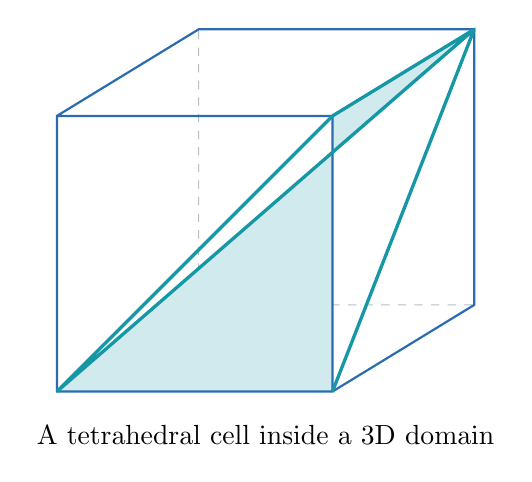
\begin{tikzpicture}[x=1cm,y=1cm]

\coordinate (A) at (0,0);\coordinate (B) at (3.5,0);\coordinate (C) at (3.5,3.5);\coordinate (D) at (0,3.5);
\coordinate (E) at (1.8,1.1);\coordinate (F) at (5.3,1.1);\coordinate (G) at (5.3,4.6);\coordinate (H) at (1.8,4.6);
\draw[FEMgray!45,dashed] (A)--(E)--(F) (E)--(H);
\fill[FEMteal!20] (A)--(B)--(C)--(G)--cycle;
\draw[FEMblue,thick] (A)--(B)--(C)--(D)--cycle (B)--(F)--(G)--(C) (D)--(H)--(G);
\draw[FEMteal,very thick] (A)--(C)--(G)--(A) (B)--(G);
\node[below,align=center] at (2.65,-.3) {A tetrahedral cell inside a 3D domain};

\end{tikzpicture}
}
\begin{columns}[t,onlytextwidth]
\column{.25\textwidth}\small
Tetrahedra replace triangles.
\column{.35\textwidth}\small
The weak form and local assembly follow the same pattern.
\column{.34\textwidth}\small
Refinement introduces unknowns much faster in 3D.
\end{columns}
\end{frame}

\section{Error estimates and convergence}
\begin{frame}{From best approximation to a convergence rate}
\begin{block}{The missing step}
C\'ea bounds FEM error by the best approximation error. We still need to know how that approximation improves as $h$ decreases.
\end{block}\[
\underbrace{\text{Stability}}_{\text{Galerkin / C\'ea}}\quad+\quad\underbrace{\text{Approximation}}_{\text{Interpolation}}\quad\Longrightarrow\quad\text{Convergence rate}.
\]\key{The convergence rate depends on mesh size, polynomial degree, and solution smoothness.}
\end{frame}

\begin{frame}{Interpolation: exact at nodes, not between them}
\begin{columns}[c,onlytextwidth]\column{.43\textwidth}
For smooth $u$, the nodal interpolant $I_hu$ matches its values at the finite element nodes.\begin{block}{Interpolant and computed solution}
$I_hu$ is an approximation tool. The computed FEM solution $u_h$ is defined by the Galerkin equations.
\end{block}
\column{.53\textwidth}
\FEMfigure[.67\textheight]{between_node_error.png}{
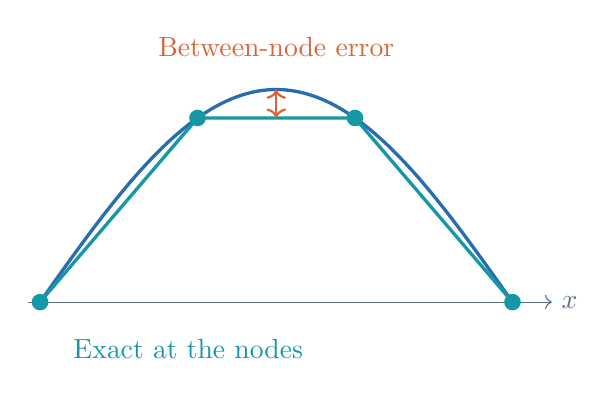
\begin{tikzpicture}[x=1cm,y=1cm]

\draw[->,FEMgray] (-.15,0)--(6.5,0) node[right] {$x$};
\draw[FEMblue,very thick,domain=0:6,samples=90] plot (\x,{2.7*sin(30*\x)});
\draw[FEMteal,very thick] (0,0)--(2,2.3383)--(4,2.3383)--(6,0);
\foreach \x/\y in {0/0,2/2.3383,4/2.3383,6/0}{\fill[FEMteal] (\x,\y) circle (3pt);}
\draw[<->,FEMorange,thick] (3,2.34)--(3,2.7);
\node[FEMorange,above,align=center] at (3,3.0) {Between-node error};
\node[FEMteal,anchor=west] at (.3,-.6) {Exact at the nodes};

\end{tikzpicture}
}
\end{columns}
\end{frame}

\begin{frame}{The basic $P_1$ interpolation estimates}
For $u\in H^2(\Omega)$ on a shape-regular mesh,\[
\begin{aligned}\|u-I_hu\|_{H^1}&\le Ch\,|u|_{H^2},\\[4mm]\|u-I_hu\|_{L^2}&\le Ch^2|u|_{H^2}.\end{aligned}
\]\key{The constant is independent of mesh size. The two norms measure different errors.}
\end{frame}

\begin{frame}{Higher degree improves the approximation order}
For sufficiently smooth $u$ and degree-$k$ elements,\[
\begin{aligned}\|u-I_hu\|_{H^1}&\lesssim h^k|u|_{H^{k+1}},\\[4mm]\|u-I_hu\|_{L^2}&\lesssim h^{k+1}|u|_{H^{k+1}}.\end{aligned}
\]\key{The higher rate requires derivatives of $u$ through order $k+1$.}
\end{frame}

\begin{frame}{Energy-error rates for the FEM solution}
Combine C\'ea's lemma with interpolation:\[
\|u-u_h\|_{H^1}\le C\|u-I_hu\|_{H^1}.
\]\begin{center}\renewcommand{\arraystretch}{1.55}
\begin{tabular}{lll}\toprule
\textbf{Element}&\textbf{Smoothness needed}&\textbf{Energy / $H^1$ error}\\\midrule
$P_1$&$u\in H^2$&$O(h)$\\
$P_2$&$u\in H^3$&$O(h^2)$\\\bottomrule
\end{tabular}\end{center}
\end{frame}

\begin{frame}{How to read a convergence plot}
\FEMfigure[.65\textheight]{lagrange_convergence_slide.png}{

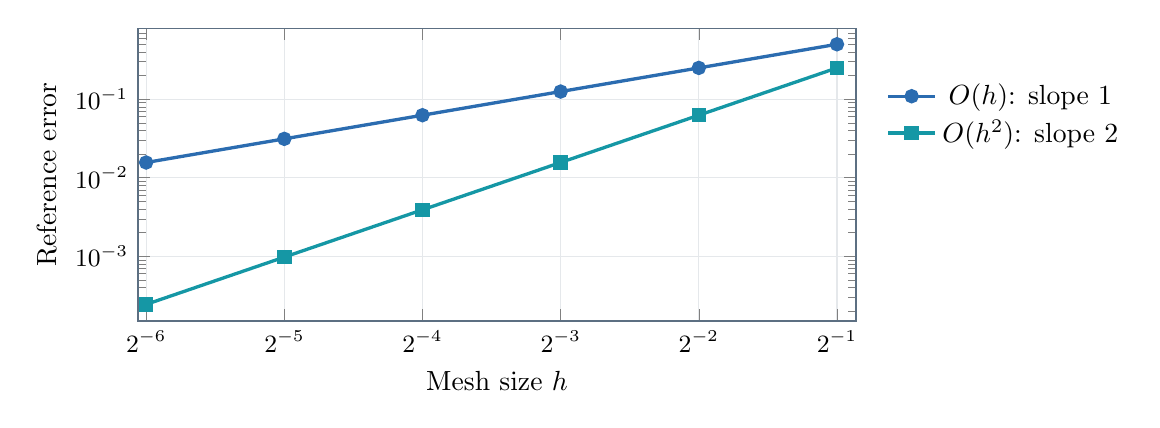
\begin{tikzpicture}
\begin{loglogaxis}[width=10.7cm,height=5.3cm,xlabel={Mesh size $h$},ylabel={Reference error},
 xmin=.015,xmax=.55,ymin=.00015,ymax=.8,grid=major,
 tick label style={font=\small},label style={font=\normalsize},
 legend style={at={(1.03,.85)},anchor=north west,draw=none,font=\normalsize},
 axis line style={FEMgray},grid style={FEMgray!16},log basis x=2,log basis y=10]
\addplot[FEMblue,very thick,mark=*] coordinates {(.5,.5)(.25,.25)(.125,.125)(.0625,.0625)(.03125,.03125)(.015625,.015625)};
\addlegendentry{$O(h)$: slope 1}
\addplot[FEMteal,very thick,mark=square*] coordinates {(.5,.25)(.25,.0625)(.125,.015625)(.0625,.00390625)(.03125,.00097656)(.015625,.00024414)};
\addlegendentry{$O(h^2)$: slope 2}
\end{loglogaxis}
\end{tikzpicture}
}\begin{center}\small\IfFileExists{lagrange_convergence_slide.png}{}{Reference slopes, not measured errors. }If $E(h)\approx Ch^p$, halving $h$ reduces the error by about $2^p$.\end{center}
\end{frame}

\begin{frame}{Regularity can limit the rate}
\begin{block}{The nominal rate has a condition}
The degree-$k$ estimate uses derivatives of $u$ up to order $k+1$. Without them, the expected rate may not appear.
\end{block}\begin{itemize}
\item Re-entrant corners and changing boundary conditions.
\item Material interfaces, rough coefficients, or singular sources.
\end{itemize}\key{Increasing polynomial degree alone does not remove a singularity.}
\end{frame}

\begin{frame}{An L-shaped domain: the re-entrant corner}
\FEMfigure[.55\textheight]{lshape_singularity_slide.png}{
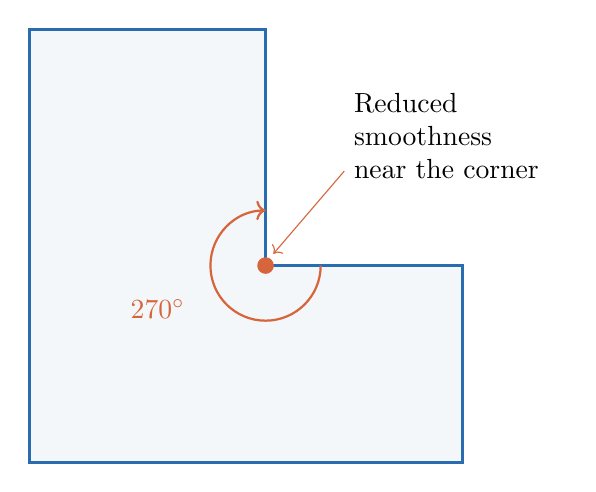
\begin{tikzpicture}[x=1cm,y=1cm]

\fill[FEMlight] (-3,-2.5)--(2.5,-2.5)--(2.5,0)--(0,0)--(0,3)--(-3,3)--cycle;
\draw[FEMblue,very thick] (-3,-2.5)--(2.5,-2.5)--(2.5,0)--(0,0)--(0,3)--(-3,3)--cycle;
\fill[FEMorange] (0,0) circle (3pt);
\draw[FEMorange,thick,->] (.7,0) arc (0:-270:.7);
\node[FEMorange,anchor=east] at (-.9,-.55) {$270^\circ$};
\node[anchor=west,align=left,text width=2.6cm] at (1,1.65) {Reduced smoothness\\near the corner};
\draw[->,FEMorange] (1.0,1.2)--(.1,.15);

\end{tikzpicture}
}
\begin{block}{A re-entrant corner}
\small
The solution may belong to $H^1$ but not $H^2$. The standard first-order $P_1$ energy estimate then loses its smoothness assumption.

Local refinement targets the small region that dominates the error.
\end{block}
\end{frame}

\begin{frame}{Why the $L^2$ error can converge faster}
\begin{exampleblock}{Aubin--Nitsche: the useful conclusion}
With sufficient primal and dual regularity,\[
\boxed{\|u-u_h\|_{L^2}\le Ch\,\|u-u_h\|_{H^1}.}
\]
\end{exampleblock}For smooth degree-$k$ FEM, this gives $O(h^{k+1})$ in $L^2$.\begin{alertblock}{The extra order is conditional}
Non-convex domains or rough coefficients can reduce the gain.
\end{alertblock}
\end{frame}

\section{A posteriori estimation and adaptivity}
\begin{frame}{Two kinds of error information}
\begin{columns}[c,onlytextwidth]\column{.48\textwidth}
\begin{block}{A priori: predict the trend}
\begin{itemize}
\item Uses $h$, degree, and solution regularity.
\item Explains asymptotic convergence rates.
\end{itemize}
\end{block}
\column{.48\textwidth}
\begin{exampleblock}{A posteriori: assess this computation}
\begin{itemize}
\item Uses the computed $u_h$ and problem data.
\item Locates where refinement is useful.
\end{itemize}
\end{exampleblock}
\end{columns}\key{The exact solution is unknown in practice; computable indicators help guide the mesh.}
\end{frame}

\begin{frame}{Element residuals: the local equation mismatch}
The exact solution satisfies $-\Delta u=f$. Inside each element, define\[
\boxed{R_K=f+\Delta u_h.}
\]\begin{exampleblock}{For affine $P_1$ elements}
$\Delta u_h=0$ inside each cell, so $R_K=f$ for the basic Poisson problem. Edge information is also needed.
\end{exampleblock}
\end{frame}

\begin{frame}{Flux jumps add the missing interface information}
\begin{columns}[c,onlytextwidth]\column{.43\textwidth}
\[
J_E=[\nabla u_h\cdot n]_E.
\]Although $u_h$ is continuous, its gradient usually changes across cell boundaries.\begin{block}{Local indicator}
Large flux jumps can signal insufficient resolution.
\end{block}
\column{.53\textwidth}
\FEMfigure[.67\textheight]{flux_jumps.png}{
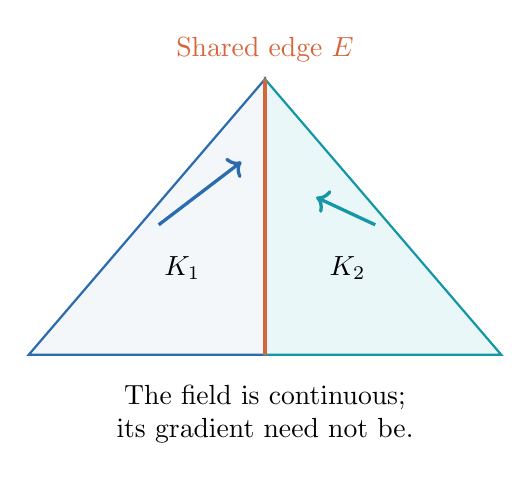
\begin{tikzpicture}[x=1cm,y=1cm]

\filldraw[fill=FEMlight,draw=FEMblue,thick] (0,0)--(3,3.5)--(3,0)--cycle;
\filldraw[fill=FEMpale,draw=FEMteal,thick] (3,0)--(3,3.5)--(6,0)--cycle;
\draw[FEMorange,very thick] (3,0)--(3,3.5);
\node[FEMorange,above] at (3,3.6) {Shared edge $E$};
\node at (1.95,1.1) {$K_1$};\node at (4.05,1.1) {$K_2$};
\draw[->,FEMblue,very thick] (1.65,1.65)--(2.7,2.45);
\draw[->,FEMteal,very thick] (4.4,1.65)--(3.65,2.0);
\node[align=center] at (3,-.75) {The field is continuous;\\its gradient need not be.};

\end{tikzpicture}
}
\end{columns}
\end{frame}

\begin{frame}{What a useful error estimator measures}
\begin{block}{Combine cell and interface information}
Each local indicator $\eta_K$ combines mesh-weighted residual and flux-jump contributions.\[
\eta=\left(\sum_K\eta_K^2\right)^{1/2}.
\]
\end{block}\begin{columns}[c,onlytextwidth]\column{.48\textwidth}
\begin{block}{Reliability}
The estimator controls the true error, up to a constant.
\end{block}
\column{.48\textwidth}
\begin{exampleblock}{Efficiency}
It also gives a lower bound for the error, up to constants and data-approximation terms.
\end{exampleblock}
\end{columns}
\end{frame}

\begin{frame}{The adaptive FEM loop}
\begin{center}
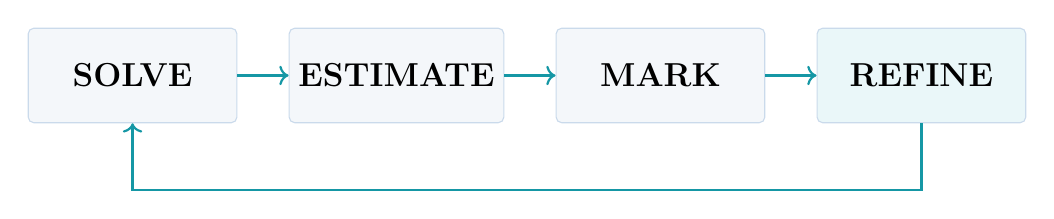
\begin{tikzpicture}[node distance=.65cm]
\tikzset{femstep/.style={draw=FEMblue!25,fill=FEMlight,rounded corners=2pt,minimum width=2.65cm,minimum height=1.2cm,align=center,font=\large\bfseries}}
\node[femstep] (s) {SOLVE}; \node[femstep,right=of s] (e) {ESTIMATE};
\node[femstep,right=of e] (m) {MARK}; \node[femstep,fill=FEMpale,right=of m] (r) {REFINE};
\draw[->,thick,FEMteal] (s)--(e);\draw[->,thick,FEMteal] (e)--(m);\draw[->,thick,FEMteal] (m)--(r);
\draw[->,thick,FEMteal] (r.south)--++(0,-.85)-|(s.south);
\end{tikzpicture}
\end{center}
\vspace{4mm}
\begin{center}\large Add unknowns where the estimated error is largest.\end{center}
\end{frame}

\begin{frame}{Uniform versus adaptive refinement}
\FEMfigure[.61\textheight]{adaptive_refinement.png}{
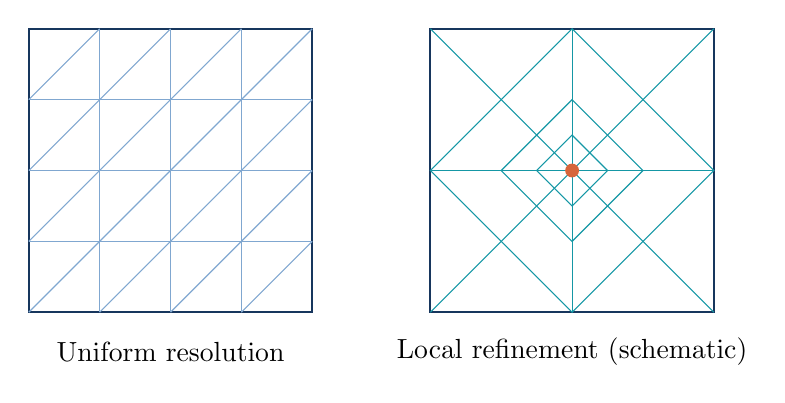
\begin{tikzpicture}[x=1cm,y=1cm]

\foreach \s in {0,5.1}{\draw[FEMnavy,thick] (\s,0) rectangle ++(3.6,3.6);}
\foreach \x in {.9,1.8,2.7}{\draw[FEMblue!60] (\x,0)--(\x,3.6);\draw[FEMblue!60] (0,\x)--(3.6,\x);}
\foreach \x in {0,.9,1.8,2.7}{\foreach \y in {0,.9,1.8,2.7}{\draw[FEMblue!60] (\x,\y)--++(.9,.9);}}
\draw[FEMteal] (5.1,0)--(8.7,3.6) (5.1,3.6)--(8.7,0);
\foreach \r in {.45,.9,1.8}{
 \draw[FEMteal] ({6.9-\r},1.8)--(6.9,{1.8+\r})--({6.9+\r},1.8)--(6.9,{1.8-\r})--cycle;}
\draw[FEMteal] (5.1,1.8)--(8.7,1.8) (6.9,0)--(6.9,3.6);
\fill[FEMorange] (6.9,1.8) circle (2.5pt);
\node at (1.8,-.5) {Uniform resolution};\node at (6.9,-.5) {Local refinement (schematic)};

\end{tikzpicture}
}\key{Uniform refinement adds resolution everywhere. Adaptivity concentrates it near difficult features.}
\end{frame}

\begin{frame}{Marking elements: a small example}
Select cells whose squared indicators account for a chosen fraction of the total.\[
\eta_K^2:\quad 16,\;9,\;4,\;1\qquad\Longrightarrow\qquad\text{total}=30.
\]\begin{exampleblock}{Target: 50\% of the estimated squared error}
The target is $15$. The largest contribution is $16$, so that element alone reaches the target.
\end{exampleblock}This illustrates bulk marking, also called D\"orfler marking.
\end{frame}

\section{Evolution PDEs: space and time}
\begin{frame}{From Poisson to the heat equation}
\[
u_t-\Delta u=f\quad\text{in }\Omega\times(0,T),
\]\[
u=0\quad\text{on }\partial\Omega,\qquad u(\cdot,0)=u_0.
\]\begin{exampleblock}{Two discretization choices}
Approximate the field in space, then advance its coefficients in time.
\end{exampleblock}
\end{frame}

\begin{frame}{The weak heat equation}
Test and integrate in space, just as for Poisson:\[
\boxed{(u_t,v)_{L^2}+a(u,v)=(f,v)_{L^2}\qquad\forall v\in H_0^1(\Omega).}
\]\begin{exampleblock}{What is new?}
The time derivative appears in an $L^2$ inner product. Time is still continuous.
\end{exampleblock}
\end{frame}

\begin{frame}{Discretize only in space}
Choose $V_h\subset H_0^1(\Omega)$ and seek $u_h(t)\in V_h$:\[
(\partial_tu_h,v_h)_{L^2}+a(u_h,v_h)=(f,v_h)_{L^2}\qquad\forall v_h\in V_h.
\]\begin{exampleblock}{Semidiscrete approximation}
The basis functions are fixed in space. Their coefficients $U_j(t)$ vary continuously in time.
\end{exampleblock}
\end{frame}

\begin{frame}{Space discretization produces an ODE system}
\[
u_h(t)=\sum_jU_j(t)\phi_j\qquad\Longrightarrow\qquad\boxed{M\dot U+AU=F.}
\]\begin{columns}[c,onlytextwidth]\column{.48\textwidth}
\begin{block}{Mass matrix}
\[
M_{ij}=(\phi_j,\phi_i)_{L^2}.
\]
\end{block}
\column{.48\textwidth}
\begin{exampleblock}{Stiffness matrix}
\[
A_{ij}=a(\phi_j,\phi_i).
\]
\end{exampleblock}
\end{columns}This is the method-of-lines viewpoint.
\end{frame}

\begin{frame}{Time levels and initial data}
\begin{columns}[c,onlytextwidth]\column{.48\textwidth}
\begin{block}{Choose the time grid}
\[
t_n=n\Delta t,\qquad U^n\approx U(t_n).
\]
\end{block}
\column{.48\textwidth}
\begin{exampleblock}{Represent the starting field}
Choose $u_h^0\in V_h$ by interpolation or projection of $u_0$.
\end{exampleblock}
\end{columns}\key{A time-stepping method advances the coefficient vector from one level to the next.}
\end{frame}

\begin{frame}{Forward Euler}
Evaluate the stiffness term at the current time level:\[
\boxed{M\frac{U^{n+1}-U^n}{\Delta t}+AU^n=F^n.}
\]\begin{itemize}
\item First order in time.
\item The update still requires handling the mass matrix $M$.
\end{itemize}\key{Its diffusion stability limit depends on the spatial mesh.}
\end{frame}

\begin{frame}{The explicit diffusion time-step restriction}
\[
\Delta t\lesssim C h^2.
\]\begin{exampleblock}{A practical consequence}
On comparable quasi-uniform meshes, halving $h$ requires roughly four times as many time steps over the same time interval.
\end{exampleblock}\begin{alertblock}{Stability is not accuracy}
A step that is stable can still be too large to resolve the time evolution.
\end{alertblock}
\end{frame}

\begin{frame}{Backward Euler}
\[
\boxed{(M+\Delta t A)U^{n+1}=MU^n+\Delta t F^{n+1}.}
\]\begin{itemize}
\item First order in time and implicit.
\item Requires a linear solve at each step.
\item Unconditionally stable in the standard energy sense for the heat equation.
\end{itemize}\key{There is no diffusion CFL limit, but accuracy still constrains the time step.}
\end{frame}

\begin{frame}{Crank--Nicolson}
Average the stiffness term between the old and new time levels:\[
M\frac{U^{n+1}-U^n}{\Delta t}+\frac12A(U^{n+1}+U^n)=F^{n+1/2}.
\]\begin{exampleblock}{Higher time accuracy}
Second order in time for sufficiently smooth solutions. Like backward Euler, it is implicit.
\end{exampleblock}
\end{frame}

\begin{frame}{Balance the spatial and temporal errors}
\[
\text{error}\lesssim C_s h^p+C_t\Delta t^q.
\]\begin{columns}[c,onlytextwidth]\column{.48\textwidth}
\begin{block}{Spatial contribution}
Controlled by mesh size, element degree, and solution smoothness.
\end{block}
\column{.48\textwidth}
\begin{exampleblock}{Temporal contribution}
Controlled by the time step and the order of the time integrator.
\end{exampleblock}
\end{columns}\key{Reducing one error much below the other adds cost with little benefit.}
\end{frame}

\begin{frame}{A worked space--time balance}
For a smooth problem with $P_1$ elements and an $L^2$-type spatial error,\begin{columns}[c,onlytextwidth]\column{.48\textwidth}
\begin{block}{Backward Euler}
\[
h^2+\Delta t\qquad\Longrightarrow\qquad\Delta t\sim h^2.
\]
\end{block}
\column{.48\textwidth}
\begin{exampleblock}{Crank--Nicolson}
\[
h^2+\Delta t^2\qquad\Longrightarrow\qquad\Delta t\sim h.
\]
\end{exampleblock}
\end{columns}\key{These are accuracy balances, not stability restrictions.}
\end{frame}

\begin{frame}{What heat diffusion looks like over time}
\FEMfigure[.60\textheight]{heat1d_theta.png}{
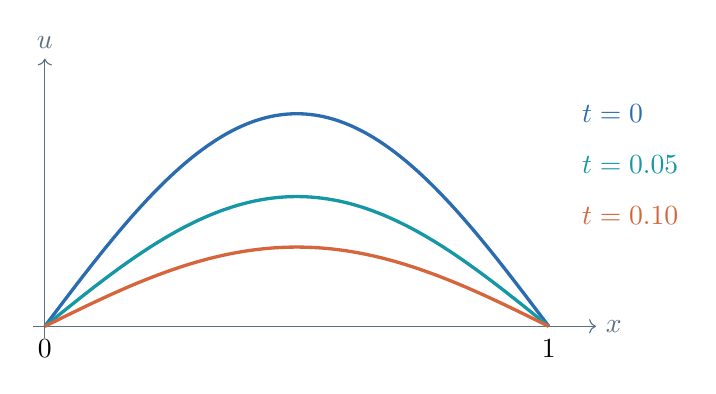
\begin{tikzpicture}[x=1cm,y=1cm]

\draw[->,FEMgray] (-.15,0)--(7,0) node[right] {$x$};
\draw[->,FEMgray] (0,-.15)--(0,3.4) node[above] {$u$};
\draw[FEMblue,very thick,domain=0:6.4,samples=90] plot (\x,{2.7*sin(180*\x/6.4)});
\draw[FEMteal,very thick,domain=0:6.4,samples=90] plot (\x,{1.6477*sin(180*\x/6.4)});
\draw[FEMorange,very thick,domain=0:6.4,samples=90] plot (\x,{1.0063*sin(180*\x/6.4)});
\node[FEMblue,anchor=west] at (6.7,2.7) {$t=0$};
\node[FEMteal,anchor=west] at (6.7,2.05) {$t=0.05$};
\node[FEMorange,anchor=west] at (6.7,1.4) {$t=0.10$};
\node[below] at (0,-.04) {$0$};\node[below] at (6.4,-.04) {$1$};

\end{tikzpicture}
}\begin{center}\small\IfFileExists{heat1d_theta.png}{Space--time evolution, solution snapshots, and temporal convergence for the 1D heat equation.}{Illustrative exact 1D profiles: $u(x,t)=e^{-\pi^2t}\sin(\pi x)$ with zero source and boundary values.}\end{center}
\end{frame}

\begin{frame}{The space--time idea extends to other PDEs}
\begin{columns}[c,onlytextwidth]\column{.43\textwidth}
\begin{block}{Diffusion}
Time stepping must respect dissipative behavior.
\end{block}
\column{.53\textwidth}
\begin{exampleblock}{Waves and transport}
Wave equations have second time derivatives; advection-dominated models may need stabilization.
\end{exampleblock}
\end{columns}\key{Reuse the workflow, but recheck stability for the new equation.}
\end{frame}

\section{Checking the solution}
\begin{frame}{Before trusting a simulation}
\begin{itemize}
\item Check the weak form and boundary conditions.
\item Check the approximation assumptions and observed convergence.
\item Use error indicators to guide resolution, not as exact errors.
\item For evolution problems, control both space and time errors.
\end{itemize}
\end{frame}

\begin{frame}{Which result answers which question?}
\begin{center}\renewcommand{\arraystretch}{1.7}
\begin{tabular}{ll}\toprule
\textbf{Question}&\textbf{Tool}\\\midrule
Does the weak problem have a stable solution? & Lax--Milgram\\
How good is the discrete approximation? & Galerkin and C\'ea\\
How fast does the error decrease? & Interpolation and regularity\\
Where should the mesh be refined? & A posteriori indicators\\\bottomrule
\end{tabular}\end{center}
\end{frame}

\begin{frame}{From the PDE to a checked solution}
\begin{block}{Formulate}
Write the weak form and choose the trial and test spaces.
\end{block}\begin{exampleblock}{Approximate}
Choose local polynomial bases and assemble the sparse system.
\end{exampleblock}\begin{block}{Verify}
Check stability, measure convergence, and estimate the remaining error.
\end{block}
\end{frame}

\end{document}
